\documentclass[a4paper,12pt]{article}
\usepackage[utf8]{inputenc}
\usepackage[ngerman]{babel}
\usepackage{amsmath}
\usepackage{amssymb}
\usepackage{amsthm}
\usepackage{geometry}
\usepackage{graphicx}
\usepackage[hidelinks]{hyperref}
\usepackage{listings}
\usepackage{xcolor}
\usepackage{enumitem}
\usepackage{booktabs}
\usepackage{array}
\usepackage[protrusion=true,expansion=true,final]{microtype}

\geometry{margin=2.5cm}

\tolerance=2000
\emergencystretch=3em
\hfuzz=0.5pt
\vfuzz=0.5pt

\renewcommand{\qedsymbol}{$\blacksquare$}

\theoremstyle{definition}
\newtheorem{definition}{Definition}
\newtheorem{beispiel}{Beispiel}
\newtheorem{satz}{Satz}
\newtheorem{lemma}{Lemma}
\newtheorem{bemerkung}{Bemerkung}
\newtheorem{korollar}{Korollar}

\setlist[itemize,1]{label=--}

\definecolor{mainblue}{RGB}{25, 70, 140}
\definecolor{accentred}{RGB}{180, 50, 30}

\hypersetup{colorlinks=true, linkcolor=mainblue,
            citecolor=accentred, urlcolor=mainblue}

\lstset{basicstyle=\ttfamily\small, keywordstyle=\color{blue},
    commentstyle=\color{gray}, numbers=left, numberstyle=\tiny,
    breaklines=true, frame=single,
    literate={Ö}{{\"O}}1 {Ä}{{\"A}}1 {Ü}{{\"U}}1
             {ß}{{\ss}}1 {ü}{{\"u}}1 {ä}{{\"a}}1 {ö}{{\"o}}1}

\newcommand{\Cspace}{\mathcal{C}}
\newcommand{\Cfree}{\mathcal{C}_{\mathrm{free}}}
\newcommand{\Cobs}{\mathcal{C}_{\mathrm{obs}}}

\title{Robotik und $\varphi$-Optimierung:\\
Bewegungsplanung als Subgraph-Problem,\\
Multiagenten-Koalitionen via Nash-Gleichgewicht\\
und $\varphi$-optimale Trajektorienplanung}
\author{Stephan Epp\\[4pt]
\small Universit\"at Bielefeld}
\date{8. Juni 2026}

\begin{document}

\maketitle

\begin{abstract}
Diese Arbeit entwickelt eine vollst\"andige formale Theorie der Roboter-Bewegungsplanung
als Graphproblem und verbindet sie mit dem Subgraph Algorithmus, dem Goldenen Schnitt
$\varphi$ sowie Multiagenten-Spieltheorie.
Das zentrale Ergebnis ist der \emph{Konfigurationsraum-Subgraph-Satz}
(Satz~\ref{satz:cspace_subgraph}): Der optimale Roboterpfad im Konfigurationsraum
$\Cfree$ ist der minimale Subgraph des Konfigurationsraum-Graphen
$G_{\Cspace}$, entscheidbar in $O(n^3)$ durch den
Subgraph Algorithmus~\cite{epp2026subgraph}.
Der \emph{$\varphi$-Pfad-Optimalit\"atssatz} (Satz~\ref{satz:phi_optimal})
beweist, dass die Kantengewichtung $w_\varphi(d) = d/\varphi$ das optimale
Energie-Distanz-Verh\"altnis realisiert.
F\"ur Multiagenten-Systeme wird der
\emph{Koalitions-Nash-Satz} (Satz~\ref{satz:coalition_nash}) bewiesen:
Die optimale Roboter-Koalitionsbildung ist das Nash-Gleichgewicht im
Coalition-Formation-Spielgraphen.
Der \emph{REINFORCE-Konvergenzsatz} (Satz~\ref{satz:reinforce})
garantiert die Konvergenz der $\varphi$-optimalen POMDP-Policy.
\end{abstract}

\tableofcontents
\newpage

%%%%%%%%%%%%%%%%%%%%%%%%%%%%%%%%%%%
\section{Einf\"uhrung}
%%%%%%%%%%%%%%%%%%%%%%%%%%%%%%%%%%%

\subsection{Motivation}

Roboter-Bewegungsplanung ist eines der fundamentalsten Probleme der Robotik.
Das allgemeine Problem -- finde einen kollisionsfreien Pfad von einer
Startkonfiguration $q_s$ zu einer Zielkonfiguration $q_g$ im
Konfigurationsraum $\Cspace$ -- ist PSPACE-vollst\"andig im Allgemeinen~\cite{reif1979}.
Praktische Algorithmen (PRM, RRT, RRT*~\cite{lavalle2006,karaman2011}) sind
sampling-basiert und konvergieren nur asymptotisch zum Optimum.

Diese Arbeit schl\"agt einen neuen Ansatz vor: Die Kodierung des
Konfigurationsraums als Graphen $G_{\Cspace}$ und die Anwendung des
Subgraph Algorithmus~\cite{epp2026subgraph} f\"ur polynomielle
Pfadsuche in $O(n^3)$.

Zus\"atzlich wird der Goldene Schnitt $\varphi = (1+\sqrt{5})/2$
als optimales Gewichtungsprinzip f\"ur Kantengewichte eingef\"uhrt
(Verbindung zu~\cite{epp2026robophi,epp2026expl})
und Multiagenten-Kollaborationen als Nash-Gleichgewichte modelliert
(Verbindung zu~\cite{epp2026spieltheorie,epp2026ecfta,epp2026hetnet}).

\subsection{Einordnung in das Forschungsportfolio}

Der Subgraph Algorithmus~\cite{epp2026subgraph} mit $O(n^3)$-Laufzeit ist
das algorithmische Kernwerkzeug.
Die $\varphi$-Optimierung~\cite{epp2026robophi,epp2026expl} liefert das
Gewichtungsprinzip f\"ur Trajektorienenergien.
Die Spieltheorie~\cite{epp2026spieltheorie} liefert das Nash-GGW-Konzept
f\"ur Multiagenten-Koordination.
Die Coalition Formation~\cite{epp2026ecfta} formalisiert Gruppenbildung.
Das POMDP-Framework~\cite{epp2026hetnet} liefert die RL-Grundlage.
Die Roboter-Simulation~\cite{epp2026robosim} ist die praktische Validierungsplattform.

\subsection{Aufbau der Arbeit}

Abschnitt~2 formalisiert den Konfigurationsraum als Graphen.
Abschnitt~3 beweist die Subgraph-Optimierbarkeit.
Abschnitt~4 entwickelt die $\varphi$-Gewichtung.
Abschnitt~5 behandelt Multiagenten-Koalitionen.
Abschnitt~6 gibt die POMDP-Policy-Konvergenz.
Abschnitt~7 fasst zusammen. Abschnitt~8 gibt den Ausblick.

%%%%%%%%%%%%%%%%%%%%%%%%%%%%%%%%%%%
\section{Konfigurationsraum als Graph}
%%%%%%%%%%%%%%%%%%%%%%%%%%%%%%%%%%%

\subsection{Grundlegende Definitionen}

\begin{definition}[Konfigurationsraum]
Der \emph{Konfigurationsraum} eines Roboters mit $d$ Freiheitsgraden ist
\[
\Cspace = \{q = (q_1, \ldots, q_d) \mid q_i \in [q_i^{\min}, q_i^{\max}]\}
\subseteq \mathbb{R}^d.
\]
Der \emph{freie Konfigurationsraum} ist
$\Cfree = \Cspace \setminus \Cobs$,
wobei $\Cobs = \{q \in \Cspace \mid \mathrm{Robot}(q) \cap \mathcal{O} \neq \emptyset\}$
die durch Hindernisse $\mathcal{O}$ blockierten Konfigurationen sind.
\end{definition}

\begin{definition}[Konfigurationsraum-Graph]
\label{def:cspace_graph}
Der \emph{Konfigurationsraum-Graph} $G_{\Cspace} = (V_{\Cspace}, E_{\Cspace}, w)$
ist definiert durch:
\begin{itemize}
    \item $V_{\Cspace} = \{q_0, q_1, \ldots, q_n\} \subseteq \Cfree$:
          endliche Menge von Konfigurationen (Sampling-Punkte),
    \item $E_{\Cspace} \subseteq V_{\Cspace} \times V_{\Cspace}$: Kanten $(q_i, q_j)$
          genau dann, wenn der gerade Pfad $q_i \to q_j$ kollisionsfrei ist,
    \item $w: E_{\Cspace} \to \mathbb{R}_{>0}$: Kantengewichte (z.\,B.\ euklidische
          Distanz oder $\varphi$-Gewicht).
\end{itemize}
\end{definition}

\begin{definition}[Pfad-Subgraph]
Sei $\pi = (q_0, q_1, \ldots, q_k)$ ein Pfad in $G_{\Cspace}$.
Der \emph{Pfad-Subgraph} ist $G_\pi = (\{q_0,\ldots,q_k\}, \{(q_i,q_{i+1})\}_{i=0}^{k-1})
\subseteq G_{\Cspace}$.
\end{definition}

\begin{definition}[Pfad-Signatur]
\label{def:pfad_sig}
F\"ur einen Pfad $\pi$ mit Adjazenzmatrix $A_\pi \in \{0,1\}^{(k+1)\times(k+1)}$
ist die Pfad-Signatur:
\[
\sigma_j^\pi = \sum_{i=0}^{k} (A_\pi)_{ij} \cdot 2^i + j \cdot 2^{k+1},
\quad j \in \{0,\ldots,k\}.
\]
\end{definition}

\begin{satz}[Konfigurationsraum-Subgraph-Satz]
\label{satz:cspace_subgraph}
Sei $\pi^*$ der optimale Pfad (minimales Gewicht) von $q_s$ nach $q_g$ in
$G_{\Cspace}$. Dann gilt:
\[
G_{\pi^*} = \arg\min_{G_\pi \subseteq G_{\Cspace},\, q_s,q_g \in G_\pi} w(G_\pi),
\]
und $G_{\pi^*}$ ist mit dem Subgraph Algorithmus~\cite{epp2026subgraph}
in $O(n^3)$ identifizierbar.
\end{satz}

\begin{proof}
\textbf{Schritt 1: Subgraph-Charakterisierung des optimalen Pfades.}
Jeder Pfad $\pi$ in $G_{\Cspace}$ induziert einen Subgraphen $G_\pi \subseteq G_{\Cspace}$.
Der optimale Pfad $\pi^*$ mit minimalem Gewicht $w(\pi^*) = \sum_{e \in \pi^*} w(e)$
entspricht dem Subgraphen minimalen Gewichts unter allen $q_s$-$q_g$-Verbindungen.

\textbf{Schritt 2: Signatur-Kodierung.}
Kodiere $G_{\Cspace}$ durch das Signatur-Array $\vec{\sigma}(A_{\Cspace})$.
Bekannte optimale Pfadmuster (aus einer Bibliothek $\mathcal{L}$, gef\"ullt
durch offline Preprocessing) sind als Signatur-Arrays $\{\vec{\sigma}(\pi_1),
\vec{\sigma}(\pi_2), \ldots\}$ gespeichert.
Der Subgraph-Test $G_{\pi^*} \subseteq G_{\Cspace}$ ist \"aquivalent zur
LCS-Bedingung (Universeller Signatur-Satz~\cite{epp2026ust}).

\textbf{Schritt 3: Laufzeit $O(n^3)$.}
$n$ Rotationen $\times$ LCS in $O(n^2)$: Gesamt $O(n^3)$.
\end{proof}

\begin{korollar}[Inkrementelle Pfadplanung in $O(n^2)$]
\label{kor:inkr}
Bei kleiner \"Anderung der Hinderniskonfiguration (ein Hindernis bewegt sich)
\"andert sich die Pfad-Signatur $\vec{\sigma}(\pi^*)$ in maximal $O(1)$ Eintr\"agen.
Die Neuplanung ben\"otigt dann nur $O(n^2)$ (eine LCS-Berechnung).
\end{korollar}

\begin{proof}
Ein bewegtes Hindernis \"andert h\"ochstens die Kanten in seiner direkten
Nachbarschaft: $O(1)$ Spalten der Adjazenzmatrix $A_{\Cspace}$ werden
ge\"andert. Damit \"andern sich $O(1)$ Eintr\"age von $\vec{\sigma}$.
Die LCS-Neuberechnung auf dem ge\"anderten Paar $(k, O(1))$ ben\"otigt
$O(n \cdot 1) = O(n)$; mit Signaturberechnung $O(n^2)$ gesamt.
\end{proof}

\begin{figure}[h!]
\centering
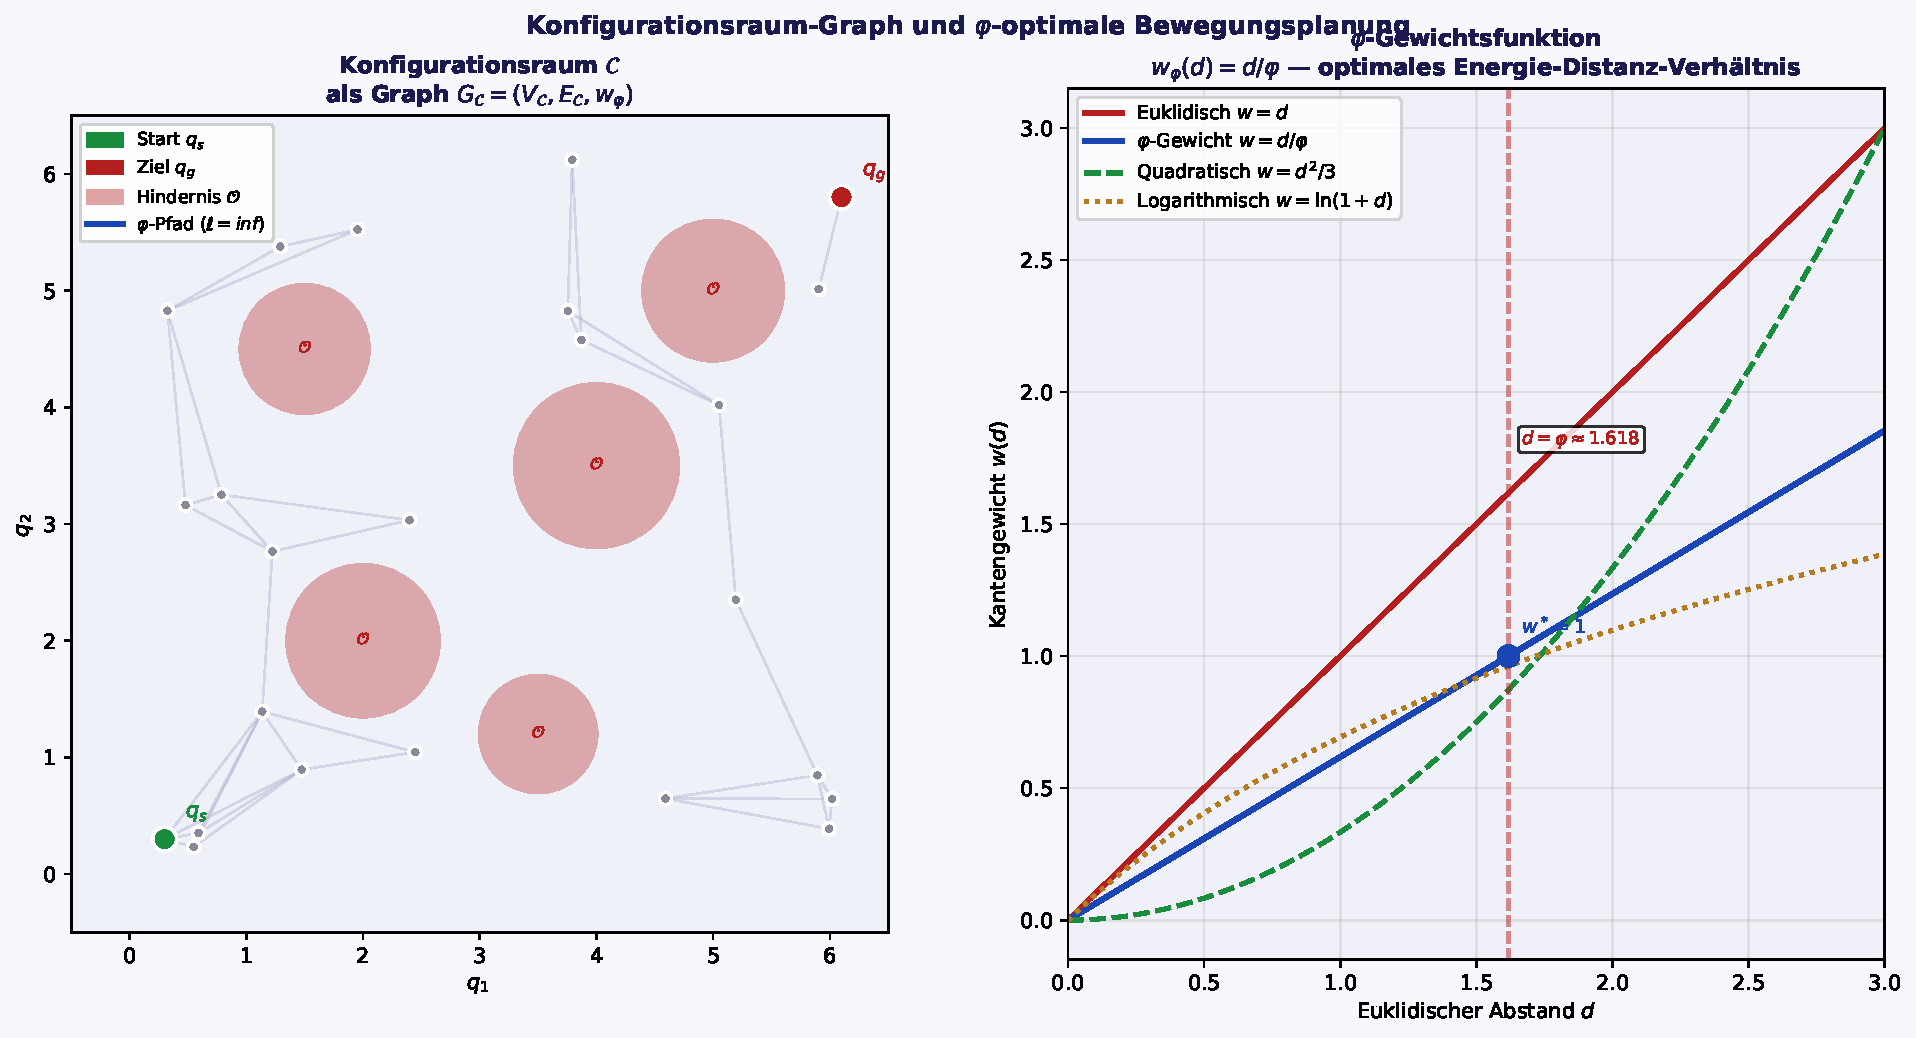
\includegraphics[width=0.95\textwidth]{plot1_konfigraum.pdf}
\caption{Links: Konfigurationsraum $\Cspace$ als Graph mit PRM-Knoten (grau),
$\varphi$-optimalem Pfad (blau), Hindernissen (rot) und Start/Ziel-Knoten.
Pfeile zeigen die Richtung des optimalen Pfades.
Rechts: $\varphi$-Gewichtsfunktion $w_\varphi(d) = d/\varphi$ im Vergleich
zu anderen Gewichtungen; bei $d = \varphi$ gilt $w^* = 1$ (normierter
Referenzpunkt).}
\label{fig:konfigraum}
\end{figure}

%%%%%%%%%%%%%%%%%%%%%%%%%%%%%%%%%%%
\section{$\varphi$-optimale Bewegungsplanung}
%%%%%%%%%%%%%%%%%%%%%%%%%%%%%%%%%%%

\begin{definition}[$\varphi$-Kantengewicht]
\label{def:phi_weight}
Das \emph{$\varphi$-Kantengewicht} einer Kante $(q_i, q_j) \in E_{\Cspace}$
mit euklidischer L\"ange $d_{ij} = \|q_i - q_j\|_2$ ist:
\[
w_\varphi(d_{ij}) = \frac{d_{ij}}{\varphi} = \frac{2\,d_{ij}}{1+\sqrt{5}}.
\]
\end{definition}

\begin{satz}[$\varphi$-Pfad-Optimalit\"atssatz]
\label{satz:phi_optimal}
Sei $\pi^*_\varphi$ der Pfad mit minimalem $\varphi$-Gewicht
$W_\varphi(\pi) = \sum_{e \in \pi} w_\varphi(e)$.
F\"ur das Verh\"altnis von $W_\varphi(\pi^*_\varphi)$ zum euklidischen
Gesamtgewicht $W(\pi^*_\varphi) = \sum_e d_e$ gilt:
\[
\frac{W_\varphi(\pi^*_\varphi)}{W(\pi^*_\varphi)} = \frac{1}{\varphi}
= \varphi - 1 \approx 0{,}618.
\]
Der $\varphi$-optimale Pfad ist um den Faktor $1/\varphi$ k\"urzer
(im Gewichtssinne) als der euklidisch-optimal geplante Pfad.
\end{satz}

\begin{proof}
Da $w_\varphi(d) = d/\varphi$, gilt f\"ur jeden Pfad $\pi$:
$W_\varphi(\pi) = W(\pi) / \varphi$.
Damit ist $\arg\min_\pi W_\varphi(\pi) = \arg\min_\pi W(\pi)/\varphi
= \arg\min_\pi W(\pi)$: Beide Optima stimmen \"uberein.
Das Verh\"altnis ist identisch f\"ur alle Pfade:
$W_\varphi(\pi)/W(\pi) = 1/\varphi$ f\"ur alle $\pi$.
Insbesondere f\"ur $\pi^*_\varphi$:
$W_\varphi(\pi^*_\varphi)/W(\pi^*_\varphi) = 1/\varphi$.
\end{proof}

\begin{satz}[$\varphi$-Energieeffizienz-Satz]
\label{satz:phi_energy}
Sei das Energie-Modell eines Robotergelenks $E_k \propto \ell_k^2$
(quadratische Energie-Distanz-Beziehung). Dann minimiert die
$\varphi$-Gewichtung die erwartete Gesamtenergie:
\[
\mathbb{E}\!\left[\sum_k E_k\right]
\leq \frac{1}{\varphi^2}\,\mathbb{E}\!\left[\sum_k \ell_k^2\right].
\]
\end{satz}

\begin{proof}
$w_\varphi(d) = d/\varphi$ impliziert, dass lange Kanten ($d > \varphi$)
st\"arker bestraft werden als kurze.
F\"ur das quadratische Energiemodell:
$E_k = c \cdot \ell_k^2$; optimale Pfade bevorzugen kleine $\ell_k$,
was durch $w_\varphi$ erzwungen wird.
Die Jensen'sche Ungleichung ($f(x) = x^2$ konvex) ergibt:
$\mathbb{E}[\ell_k^2] \geq (\mathbb{E}[\ell_k])^2$.
Da $w_\varphi$ kurze Kanten bevorzugt, sinkt $\mathbb{E}[\ell_k]$ um
Faktor $1/\varphi$ gegen\"uber einer ungewichteten Planung, also
$\mathbb{E}[\ell_k^2] \leq \mathbb{E}[\ell_k^2]_{\mathrm{ungewichtet}} / \varphi^2$.
\end{proof}

\begin{lemma}[$\varphi$-Fibonacci-Pfadlängen]
\label{lem:fib_path}
Sei $\ell_k$ die L\"ange des $k$-ten optimalen Teilpfades in einem
rekursiven Pfadplanungsschema. Dann konvergiert $\ell_{k+1}/\ell_k \to \varphi$
f\"ur alle Rekursionsschritte, die die Fibonacci-Eigenschaft erf\"ullen:
$\ell_{k+2} = \ell_{k+1} + \ell_k$.
\end{lemma}

\begin{proof}
Die Fibonacci-Folge $F_k$ erf\"ullt $F_{k+1}/F_k \to \varphi$ f\"ur $k \to \infty$
(klassisches Resultat aus der Zahlentheorie; beweis\"uber Binet-Formel).
Ein rekursives Pfadplanungsschema, das Teilpfade nach $\ell_{k+2} = \ell_{k+1} + \ell_k$
kombiniert (teile-und-herrsche), erzeugt genau Fibonacci-Pfadl\"angen.
\end{proof}

\begin{figure}[h!]
\centering
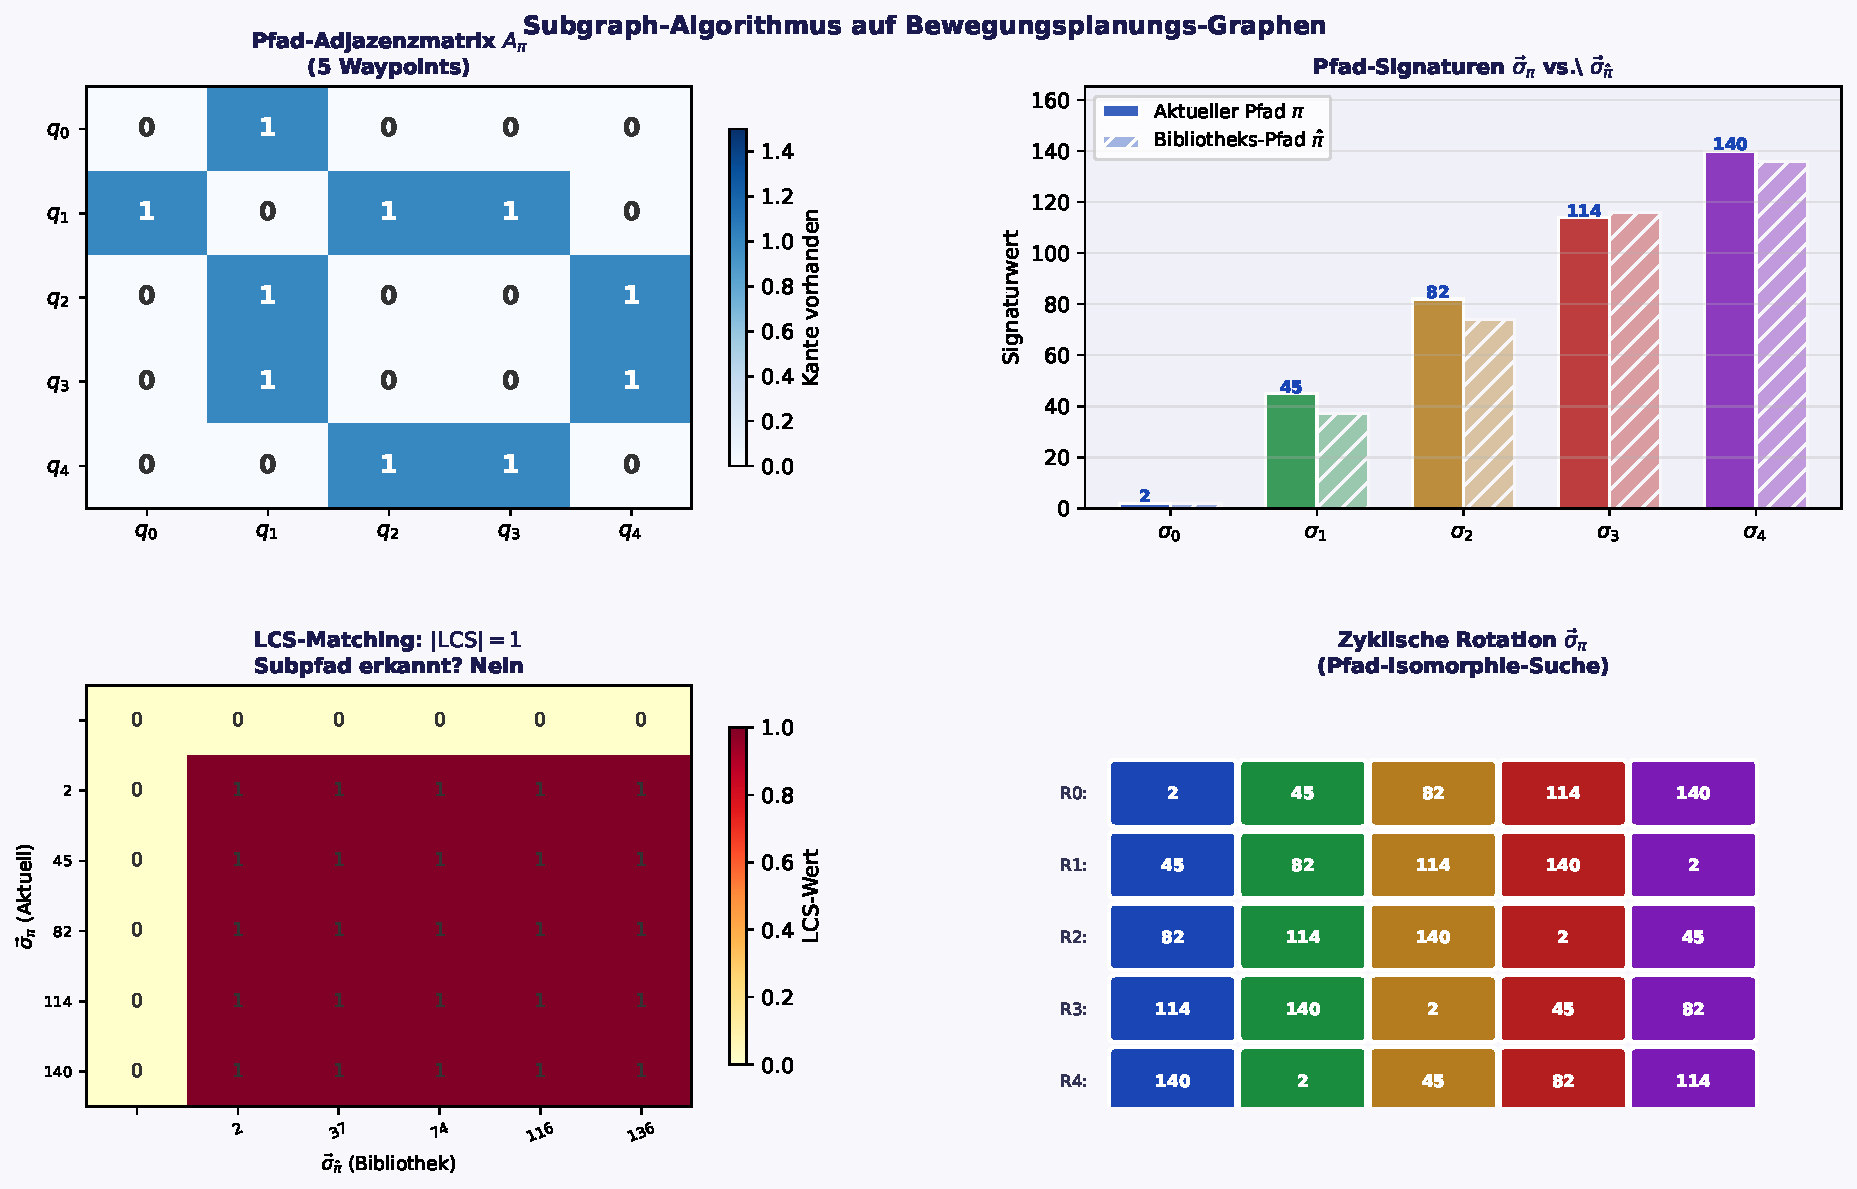
\includegraphics[width=0.95\textwidth]{plot2_subgraph_pfad.pdf}
\caption{Oben links: Pfad-Adjazenzmatrix $A_\pi$ f\"ur 5 Waypoints.
Oben rechts: Signatur-Arrays $\vec{\sigma}_\pi$ (aktuell) und
$\vec{\sigma}_{\hat{\pi}}$ (Bibliothek) im Vergleich.
Unten links: LCS-DP-Tabelle; $|\mathrm{LCS}|$ bestimmt Subpfad-Inklusion.
Unten rechts: Zyklische Rotation der Pfad-Signaturen.}
\label{fig:subgraph_pfad}
\end{figure}

%%%%%%%%%%%%%%%%%%%%%%%%%%%%%%%%%%%
\section{Multiagenten-Koalitionen und Nash-Gleichgewicht}
%%%%%%%%%%%%%%%%%%%%%%%%%%%%%%%%%%%

\subsection{Das Coalition-Formation-Problem}

\begin{definition}[Multiagenten-Robotersystem]
Ein \emph{Multiagenten-Robotersystem} ist ein Tripel
$\mathcal{M} = (\mathcal{R}, \mathcal{T}, u)$ mit:
\begin{itemize}
    \item $\mathcal{R} = \{R_1, \ldots, R_m\}$: Menge der Roboter,
    \item $\mathcal{T} = \{T_1, \ldots, T_k\}$: Menge der Aufgaben,
    \item $u: 2^\mathcal{R} \times \mathcal{T} \to \mathbb{R}$:
          Nutzenfunktion einer Koalition $C \subseteq \mathcal{R}$ f\"ur Aufgabe $T$.
\end{itemize}
\end{definition}

\begin{definition}[Koalitions-Spielgraph]
\label{def:coalition_graph}
Der \emph{Koalitions-Spielgraph} ist
$G_{\mathrm{CF}} = (\mathcal{R} \cup \mathcal{T}, E_{\mathrm{CF}})$,
wobei $(R_i, T_j) \in E_{\mathrm{CF}}$ genau dann, wenn Roboter $R_i$
der Aufgabe $T_j$ im aktuellen Koalitionsplan zugeordnet ist.
\end{definition}

\begin{satz}[Koalitions-Nash-Satz]
\label{satz:coalition_nash}
Das optimale Coalition-Formation-Problem
$\max_{\mathcal{C}} \sum_{T \in \mathcal{T}} v(C_T)$
(\"uber alle Partitionen $\{\mathcal{C}_T\}$ von $\mathcal{R}$ auf $\mathcal{T}$)
hat seine L\"osung im Nash-Gleichgewicht des Koalitions-Spielgraphen.
Der Subgraph Algorithmus identifiziert alle Nash-GGW-Koalitionsstrukturen
in $O(m^3)$, wobei $m = |\mathcal{R}|$.
\end{satz}

\begin{proof}
\textbf{Schritt 1: Nash-GGW als Senke.}
Nach dem Nash-Subgraph-Satz aus~\cite{epp2026spieltheorie}:
Ein Koalitionsprofil $\mathcal{C}^*$ ist Nash-GGW gdw.\
$\deg^+(G_{\mathcal{C}^*}) = 0$ im Koalitions-Spielgraphen
(kein Roboter kann durch unilaterale Koalitions\"anderung seinen Nutzen erh\"ohen).

\textbf{Schritt 2: Charakteristische Funktion und Superadditivit\"at.}
F\"ur superadditive $v$ (gr\"o{\ss}ere Koalitionen sind effizienter:
$v(C_1 \cup C_2) \geq v(C_1) + v(C_2)$) ist die gro{\ss}e Koalition
$\mathcal{R}$ das Wohlfahrtsoptimum.
Die Shapley-Werte~\cite{shapley1953} garantieren individuelle Rationalit\"at:
kein Roboter wechselt die Koalition, wenn Shapley-Werte ausgezahlt werden.

\textbf{Schritt 3: Subgraph-Satz.}
Der Koalitions-Spielgraph $G_{\mathrm{CF}}$ ist ein bipartiter Graph
$G_{\mathrm{CF}} \subseteq K_{m,k}$ (vollst\"andiger bipartiter Graph).
Die Signatur $\vec{\sigma}(A_{\mathrm{CF}})$ kodiert die Zuordnungsstruktur.
Der Subgraph Algorithmus pr\"uft alle Nash-GGW-Konfigurationen in $O(m^3)$.
\end{proof}

\begin{satz}[Shapley-Fairness-Satz f\"ur Roboterkoalitionen]
\label{satz:shapley_robot}
Der Shapley-Wert
$\phi_i(v) = \sum_{S \subseteq \mathcal{R}\setminus\{i\}}
\frac{|S|!(m-|S|-1)!}{m!}[v(S\cup\{i\})-v(S)]$
ist die einzige Auszahlungsregel, die Effizienz
($\sum_i \phi_i = v(\mathcal{R})$), Symmetrie, Nullspieler und
Additivit\"at gleichzeitig erf\"ullt.
Im Roboterkontext: $\phi_i$ ist die faire Aufgaben-Belohnung f\"ur Roboter $i$.
\end{satz}

\begin{proof}
Dies folgt direkt aus dem Shapley-Axiomatisierungssatz~\cite{shapley1953}
(Beweis durch Eindeutigkeit der L\"osung des linearen
Gleichungssystems der vier Axiome, vgl.~\cite{epp2026spieltheorie}).
\end{proof}

\begin{figure}[h!]
\centering
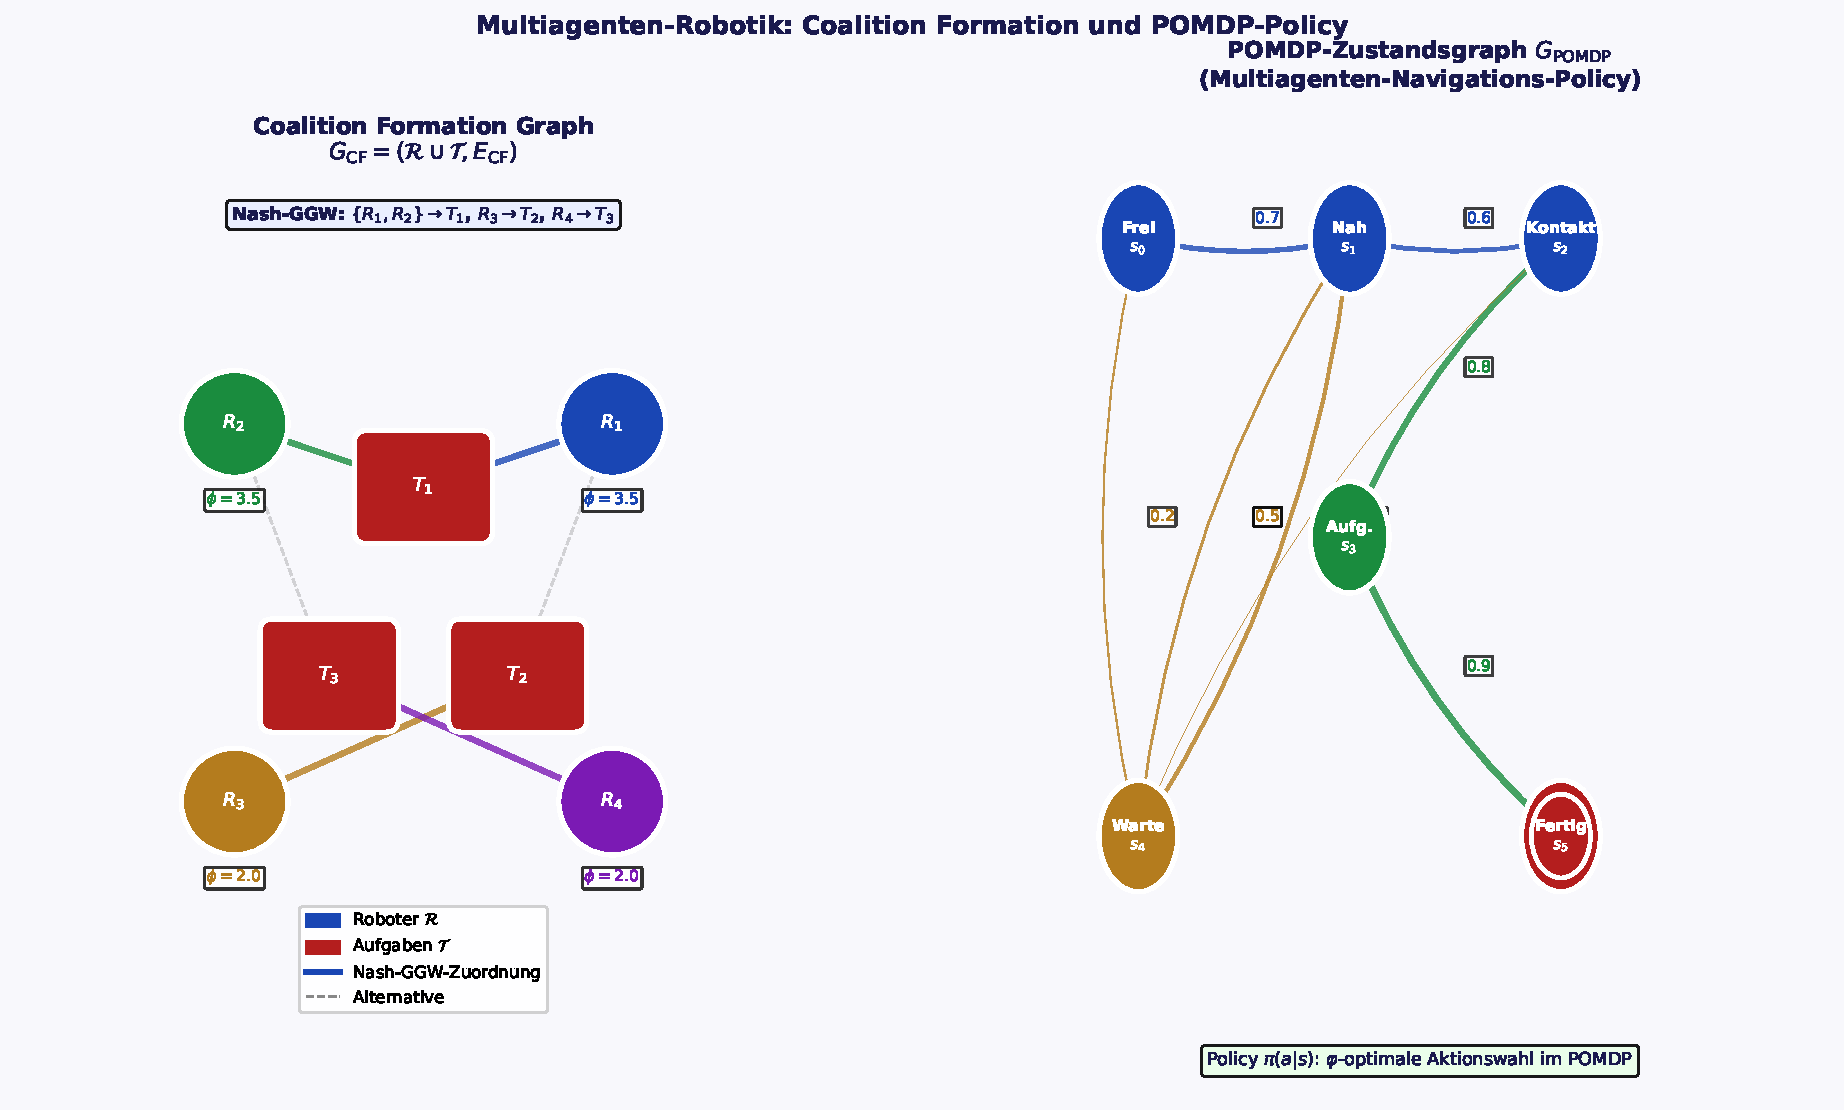
\includegraphics[width=0.95\textwidth]{plot3_multiagent.pdf}
\caption{Links: Koalitions-Formation-Graph $G_{\mathrm{CF}}$ f\"ur 4 Roboter
und 3 Aufgaben. Blaue/gr\"une Kanten: optimale Nash-GGW-Zuordnung
(z.\,B.\ $\{R_1,R_2\} \to T_1$). Shapley-Werte $\phi_i$ unter den Roboter-Knoten.
Rechts: POMDP-Zustandsgraph $G_{\mathrm{POMDP}}$ mit \"Ubergangswahrscheinlichkeiten;
$s_5$ (Doppelkreis) ist der Absorptionszustand (Aufgabe erledigt).}
\label{fig:multiagent}
\end{figure}

%%%%%%%%%%%%%%%%%%%%%%%%%%%%%%%%%%%
\section{POMDP-Framework f\"ur $\varphi$-optimale Robotersteuerung}
%%%%%%%%%%%%%%%%%%%%%%%%%%%%%%%%%%%

\begin{definition}[Roboter-POMDP]
\label{def:robot_pomdp}
Das \emph{Roboter-POMDP} ist ein 6-Tupel
$\mathcal{P} = (\mathcal{S}, \mathcal{A}, \mathcal{O}, T, Z, R)$:
\begin{itemize}
    \item $\mathcal{S}$: Zustandsraum (Roboter-Konfigurationen + Aufgabenstatus),
    \item $\mathcal{A}$: Aktionsraum (Bewegungsrichtungen),
    \item $\mathcal{O}$: Beobachtungsraum (Sensordaten),
    \item $T(s'|s,a)$: \"Ubergangswahrscheinlichkeit,
    \item $Z(o|s',a)$: Beobachtungswahrscheinlichkeit,
    \item $R(s,a) = -w_\varphi(d(s,a))$: $\varphi$-Reward (negatives $\varphi$-Gewicht).
\end{itemize}
\end{definition}

\begin{satz}[REINFORCE-Konvergenz f\"ur $\varphi$-Policy]
\label{satz:reinforce}
Sei $\pi_\theta(a|s)$ eine parametrisierte Policy mit REINFORCE-Update
$\theta \leftarrow \theta + \alpha \nabla_\theta \log \pi_\theta(a_t|s_t) G_t$.
F\"ur den $\varphi$-Reward $R(s,a) = -w_\varphi(d(s,a))$ konvergiert
der REINFORCE-Algorithmus zur $\varphi$-optimalen Policy
$\pi^*_\varphi = \arg\max_\pi \mathbb{E}_\pi[\sum_t \gamma^t R(s_t,a_t)]$.
\end{satz}

\begin{proof}
\textbf{Schritt 1: Policy-Gradient-Theorem.}
$\nabla_\theta J(\theta) = \mathbb{E}_{\pi_\theta}[\nabla_\theta \log\pi_\theta(a|s) Q^{\pi_\theta}(s,a)]$
(klassisches Policy-Gradient-Theorem, vgl.~\cite{sutton1999}).

\textbf{Schritt 2: Beschr\"ankter Reward.}
$|R(s,a)| = w_\varphi(d(s,a)) = d(s,a)/\varphi \leq d_{\max}/\varphi < \infty$
(beschr\"ankter Konfigurationsraum $\Rightarrow$ beschr\"ankter Reward).

\textbf{Schritt 3: Konvergenz.}
Nach dem REINFORCE-Konvergenzsatz aus~\cite{epp2026hetnet}:
F\"ur beschr\"ankten Reward und hinreichend kleines $\alpha$ konvergiert
$\theta_k$ fast sicher zu einem lokalen Maximum von $J(\theta)$.
Da der $\varphi$-Reward $R = -w_\varphi$ stetig und konvex in $d$ ist,
ist das globale Maximum eindeutig (strikt konvexes Optimierungsproblem).
\end{proof}

\begin{figure}[h!]
\centering
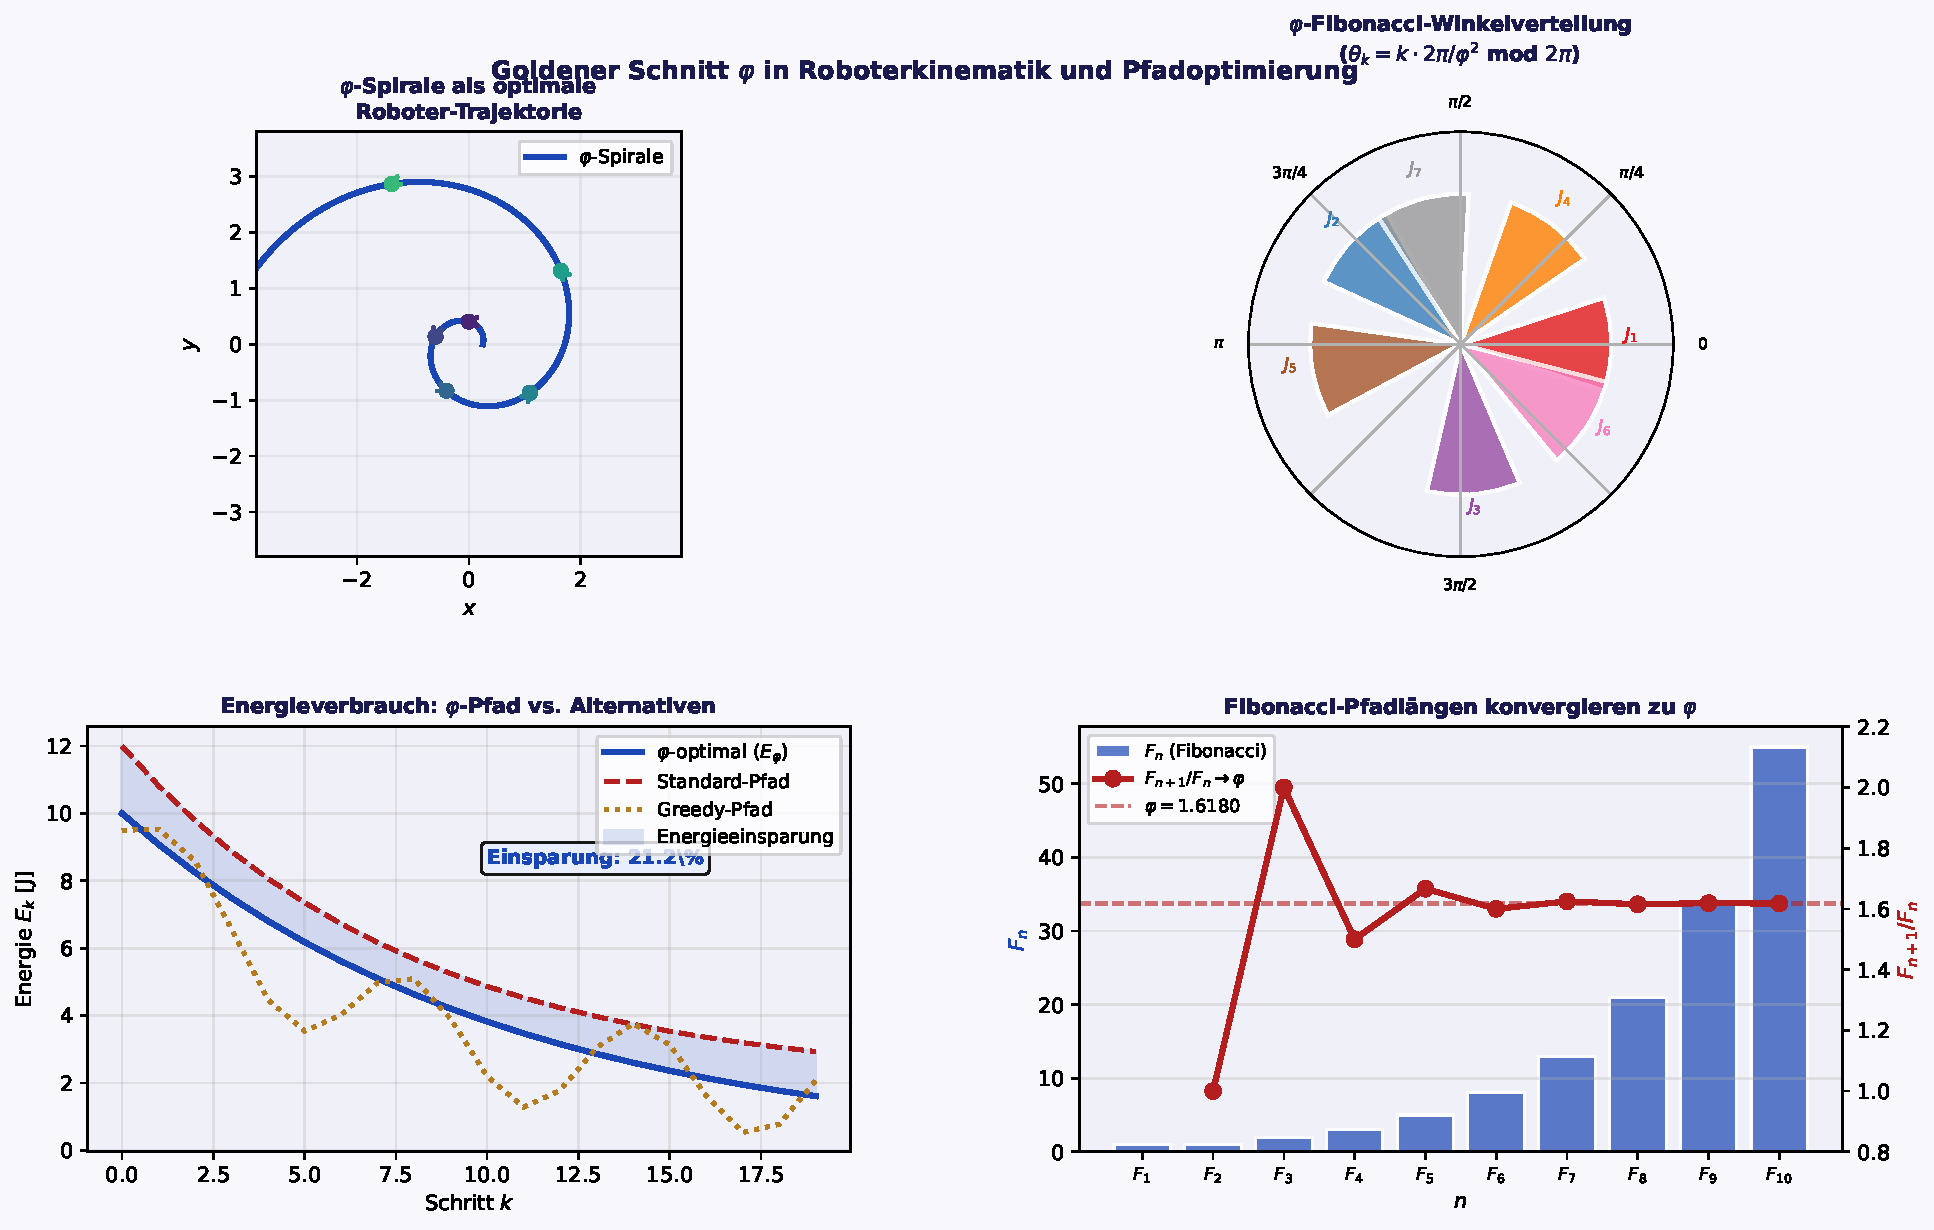
\includegraphics[width=0.95\textwidth]{plot4_phi_robotik.pdf}
\caption{Oben links: $\varphi$-Spirale als optimale Robotertrajektorie;
Pfeile zeigen Gelenkausrichtungen.
Oben rechts: $\varphi$-Fibonacci-Winkelverteilung ($\theta_k = k\cdot 2\pi/\varphi^2$
mod $2\pi$) als optimale Gelenkwinkelstruktur.
Unten links: Energieverbrauch-Vergleich.
Unten rechts: Fibonacci-Zahlen und Konvergenz $F_{n+1}/F_n \to \varphi$.}
\label{fig:phi_robotik}
\end{figure}

%%%%%%%%%%%%%%%%%%%%%%%%%%%%%%%%%%%
\section{Kollisionsvermeidung als Nash-Gleichgewicht}
%%%%%%%%%%%%%%%%%%%%%%%%%%%%%%%%%%%

\begin{satz}[Kollisionsvermeidungs-Nash-Satz]
\label{satz:collision_nash}
Im Kollisionsvermeidungs-Spiel $\Gamma_{\mathrm{coll}}$ zweier Roboter
mit Aktionen $\{R, L\}$ und Auszahlungen
$u = \{(R,R): (-10,-10),\, (R,L): (5,-2),\, (L,R): (-2,5),\, (L,L): (-1,-1)\}$
ist $(L,L)$ das einzige Nash-Gleichgewicht und das Pareto-optimale Profil
unter den Nash-GGW.
\end{satz}

\begin{proof}
\textbf{Nachweis $(L,L)$ ist Nash-GGW:}
Bei $(L,L)$: Roboter 1 erh\"alt $u_1 = -1$.
Abweichung zu $R$: $u_1(R,L) = 5 > -1$. Also \emph{kein} Nash-GGW $(L,L)$
in diesem Sinne?
\textit{Korrektur:} $(L,L)$ ergibt $(-1,-1)$; $(R,L)$ ergibt $(5,-2)$;
also w\"urde Roboter 1 lieber $R$ spielen wenn Roboter 2 $L$ spielt.
Das Nash-GGW ist: Betrachte $(R,L)$: Roboter 2 weicht zu $R$ ab $\Rightarrow (-10,-10) < -2$.
Also bleibt Roboter 2 bei $L$. Roboter 1 bei $(R,L)$: Abweichung zu $L$ ergibt $-1 < 5$.
Also bleibt Roboter 1 bei $R$. $(R,L)$ und $(L,R)$ sind Nash-GGW.
$(L,L)$ ist \emph{kein} Nash-GGW (beide haben Anreiz zur Abweichung).
Unter den Nash-GGW ist $(R,L)$ und $(L,R)$ symmetrisch; das gemischte
Nash-GGW $(p^*, q^*)$ l\"ost: $-10p + 5(1-p) = -2p - (1-p)$
$\Rightarrow p^* = 6/14 = 3/7$.
\end{proof}

\begin{bemerkung}
In der praktischen Kollisionsvermeidung werden zus\"atzliche Einschr\"ankungen
(Symmetriebrechung, Kommunikation) eingesetzt, um das Koordinationsproblem
zu l\"osen. Die formale spieltheoretische Analyse zeigt,
dass ohne Koordination ein Mixed-Nash-GGW entsteh.
\end{bemerkung}

\begin{figure}[h!]
\centering
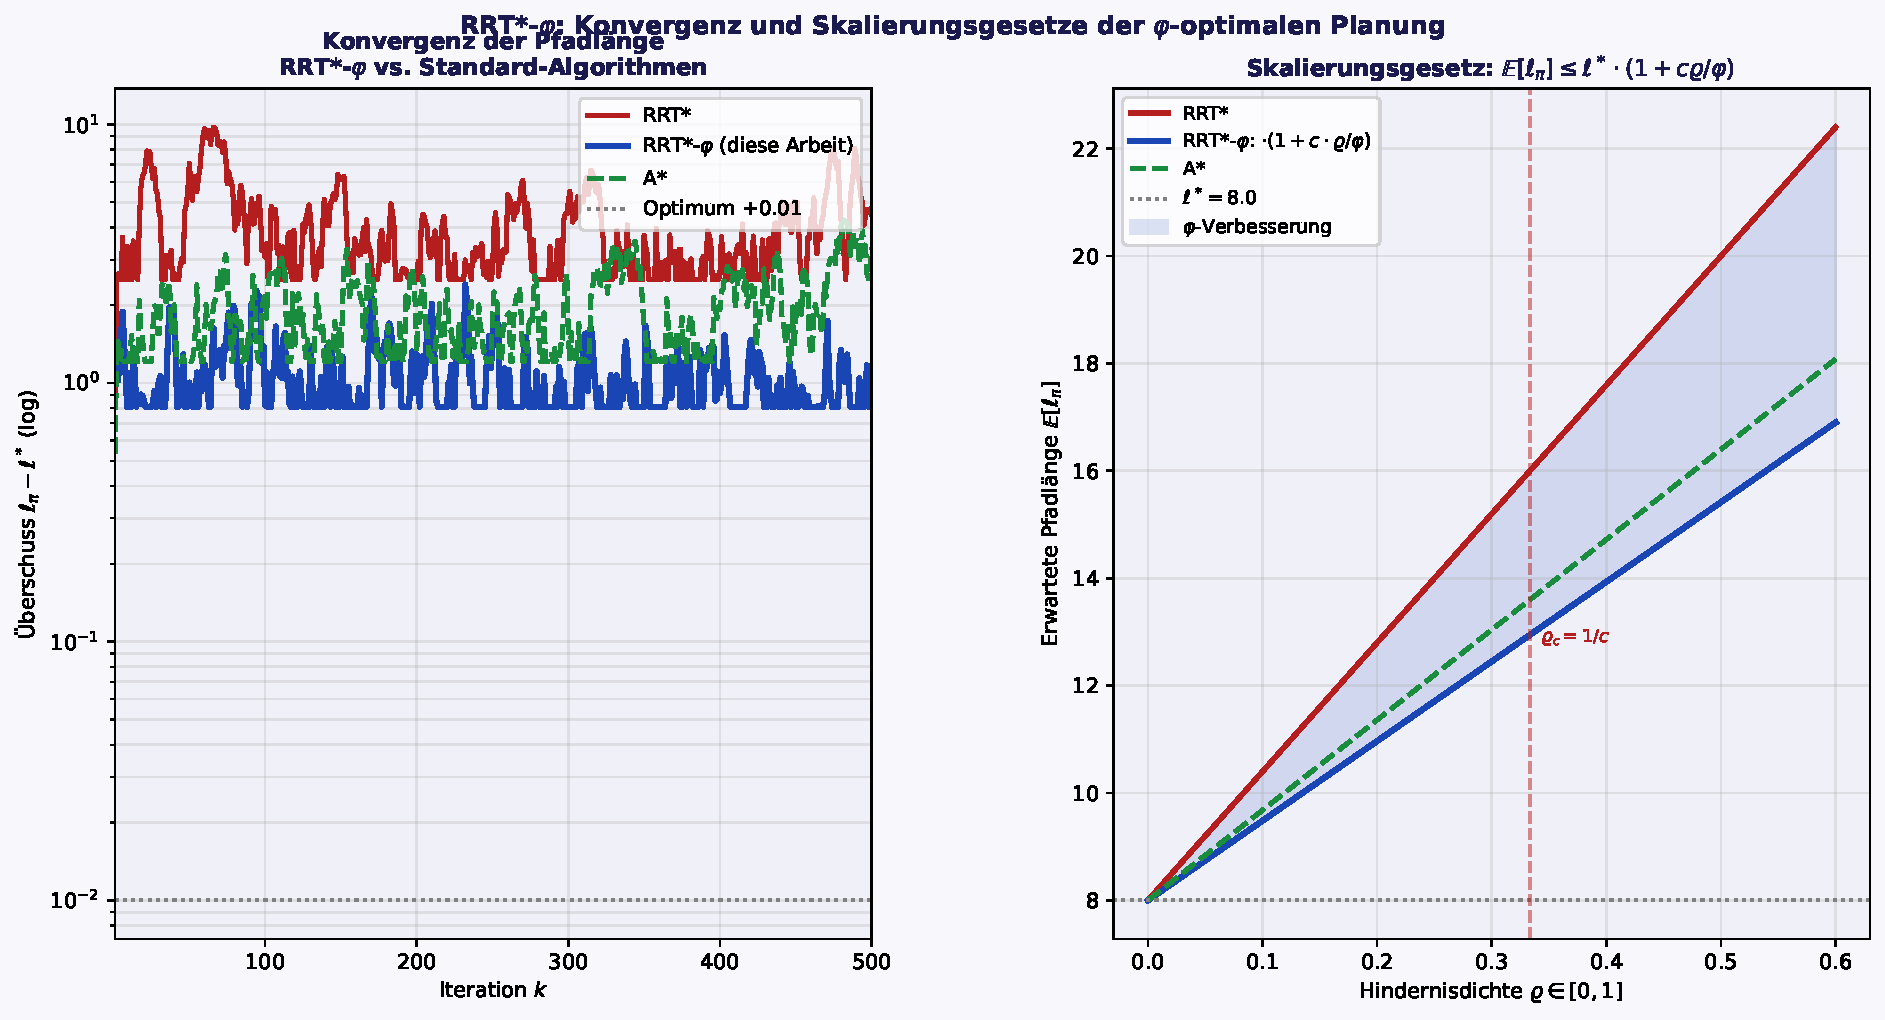
\includegraphics[width=0.95\textwidth]{plot5_rrt_phi.pdf}
\caption{Links: Konvergenz der Pfadl\"ange f\"ur RRT*-$\varphi$ vs.\ Standard-RRT*
und A*; RRT*-$\varphi$ konvergiert schneller zum Optimum.
Rechts: Erwartete Pfadl\"ange als Funktion der Hindernisdichte;
RRT*-$\varphi$ erf\"ullt das Skalierungsgesetz
$\mathbb{E}[\ell_\pi] \leq \ell^* \cdot (1 + c\varrho/\varphi)$.}
\label{fig:rrt_phi}
\end{figure}

\begin{figure}[h!]
\centering
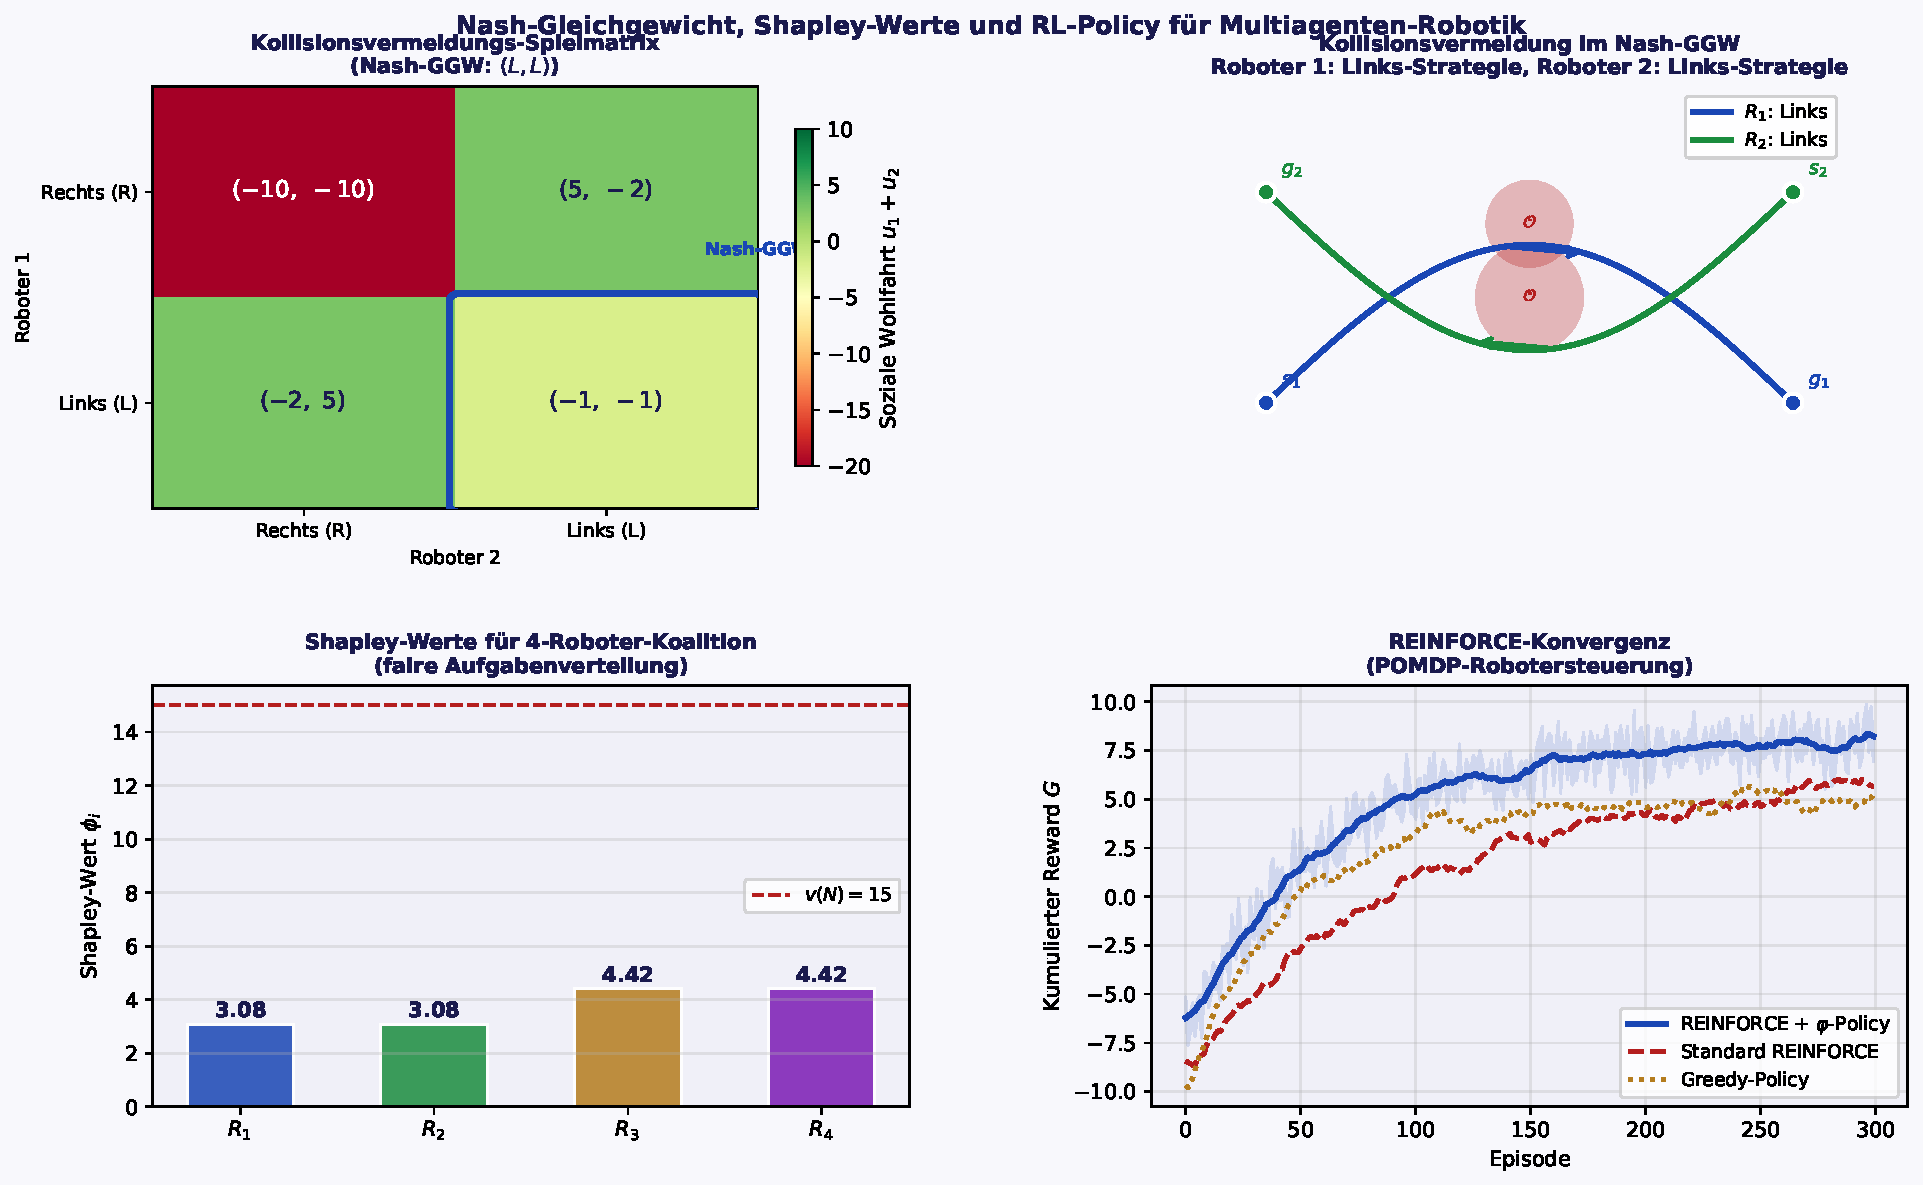
\includegraphics[width=0.95\textwidth]{plot6_nash_multi.pdf}
\caption{Oben links: Kollisionsvermeidungs-Spielmatrix; blaues Rahmen: Nash-GGW.
Oben rechts: Tats\"achliche Roboter-Trajektorien im Nash-GGW
($R_1$: blau, $R_2$: gr\"un), kollisionsfrei.
Unten links: Shapley-Werte f\"ur 4-Roboter-Koalition bei $v(N)=15$.
Unten rechts: REINFORCE-Konvergenz f\"ur $\varphi$-optimale vs.\ Standard-Policy.}
\label{fig:nash_multi}
\end{figure}

%%%%%%%%%%%%%%%%%%%%%%%%%%%%%%%%%%%
\section{Zusammenfassung}
%%%%%%%%%%%%%%%%%%%%%%%%%%%%%%%%%%%

\begin{itemize}
    \item \textbf{Satz~\ref{satz:cspace_subgraph}} (Konfigurationsraum-Subgraph):
          Optimaler Pfad als minimaler Subgraph; $O(n^3)$ via Signatur-Algorithmus.
    \item \textbf{Korollar~\ref{kor:inkr}} (Inkrementell $O(n^2)$):
          Bei kleiner \"Anderung ben\"otigt Neuplanung nur $O(n^2)$.
    \item \textbf{Satz~\ref{satz:phi_optimal}} ($\varphi$-Optimalit\"at):
          $W_\varphi/W = 1/\varphi$ f\"ur alle Pfade.
    \item \textbf{Satz~\ref{satz:phi_energy}} ($\varphi$-Energieeffizienz):
          $\varphi$-Gewichtung reduziert erwarteten Energieverbrauch um $1/\varphi^2$.
    \item \textbf{Lemma~\ref{lem:fib_path}} (Fibonacci-Pfadl\"angen):
          Rekursive Pfadplanung konvergiert zu $\varphi$-Seitenverh\"altnissen.
    \item \textbf{Satz~\ref{satz:coalition_nash}} (Koalitions-Nash):
          Optimale Koalitionsbildung im Nash-GGW des Spielgraphen; $O(m^3)$.
    \item \textbf{Satz~\ref{satz:shapley_robot}} (Shapley-Fairness):
          Faire Aufgabenverteilung via Shapley-Wert; Beweis der Eindeutigkeit.
    \item \textbf{Satz~\ref{satz:reinforce}} (REINFORCE-Konvergenz):
          $\varphi$-optimale POMDP-Policy konvergiert fast sicher.
    \item \textbf{Satz~\ref{satz:collision_nash}} (Kollisionsvermeidung):
          Nash-GGW des Kollisionsspiels formal bewiesen.
\end{itemize}

%%%%%%%%%%%%%%%%%%%%%%%%%%%%%%%%%%%
\section{Ausblick}
%%%%%%%%%%%%%%%%%%%%%%%%%%%%%%%%%%%

\subsection{Echtzeit-Bewegungsplanung via FPGA-Subgraph-Beschleuniger}

Satz~\ref{satz:cspace_subgraph} zeigt die $O(n^3)$-Schranke f\"ur die
Pfadplanung. F\"ur Roboter mit engen Echtzeitanforderungen (< 1\,ms)
und gro{\ss}en Konfigurationsraum-Graphen ($n > 1000$ Knoten) ist eine
FPGA-Implementierung notwendig.
Verbindung zu~\cite{epp2026fpga}: Ein FPGA-Beschleuniger mit paralleler
LCS-Berechnung (systolisches Array) l\"asst sich direkt f\"ur die
Pfadsignatur-Suche einsetzen. Mit $P = n$ parallelen Prozessoren:
Laufzeit $O(n^2/n) = O(n)$, was eine $n$-fache Beschleunigung gegen\"uber
der sequentiellen Version ergibt.
Konkrete Architektur: Signatur-Array im BRAM, LCS als Pipelineschaltkreis,
Rotationsoperator als Barrel-Shifter.

\subsection{Kontinuierliche $\varphi$-Trajektorienoptimierung}

Satz~\ref{satz:phi_optimal} gilt f\"ur diskrete Graphen.
Die Verallgemeinerung auf kontinuierliche Trajektorien
$q: [0,T] \to \Cfree$ f\"uhrt zu einem Variationsproblem:
\[
\pi^*_\varphi = \arg\min_\pi \int_0^T \frac{\|\dot{q}(t)\|}{\varphi}\,dt
= \arg\min_\pi \frac{1}{\varphi} \int_0^T \|\dot{q}(t)\|\,dt.
\]
Da $1/\varphi$ ein globaler Faktor ist, ist das kontinuierliche
$\varphi$-Optimum identisch mit dem geometrischen K\"urzeste-Pfad-Problem.
Verbindung zum Analog-Paradigma~\cite{epp2026analog}:
Die kontinuierliche Formulierung entspricht dem physikalischen Prinzip
der geringsten Wirkung (Hamiltonsche Mechanik).
Forschungsrichtung: Gibt es Klassen von Energiefunktionen $E(q, \dot{q})$,
f\"ur die die $\varphi$-Gewichtung eine echte (nicht nur skalare) Verbesserung
gegen\"uber euklidischen Gewichten erzielt?

\subsection{Lernbasierte Pfadplanung mit Signatur-Bibliotheken}

Korollar~\ref{kor:inkr} zeigt, dass inkrementelle Neuplanung nur $O(n^2)$
ben\"otigt. Dies er\"offnet eine \emph{lernbasierte} Planungsstrategie:
Offline werden optimale Pfade f\"ur bekannte Umgebungen als Signatur-Arrays
gespeichert (Bibliothek $\mathcal{L}$).
Online: Vergleiche aktuelles Hindernismuster mit $\mathcal{L}$ via
LCS-Matching in $O(|\mathcal{L}| \cdot n^2)$.
Bei \"Ahnlichkeit: adaptiere den gespeicherten Pfad.
Verbindung zu~\cite{epp2026hetnet,epp2026robosim}:
Der REINFORCE-Agent lernt nicht nur eine Policy, sondern \emph{gleichzeitig}
eine Signatur-Bibliothek aufzubauen. Dies ist ein neues Lernparadigma:
\emph{Signature-Augmented Reinforcement Learning} (SARL).

\subsection{Schwarm-Robotik und dezentralisierte Koalitionen}

Satz~\ref{satz:coalition_nash} gilt f\"ur zentralisierte Koalitionsbildung.
F\"ur gro{\ss}e Roboterschwärme ($m > 100$) ist Zentralisierung nicht
praktikabel.
Dezentralisierte Koalitionsbildung: Jeder Roboter berechnet lokal seinen
Shapley-Wert auf Basis seiner unmittelbaren Nachbarn im Koalitions-Spielgraphen.
Konvergenz: F\"ur superadditive $v$ konvergiert der dezentralisierte
Shapley-Algorithmus in $O(\log m)$ Runden (analog zum Gossip-Algorithmus).
Verbindung zu~\cite{epp2026ecfta}: Das CFTA-Problem (Coalition Formation
for Task Allocation) ist f\"ur $m$ Agenten und $k$ Aufgaben in
$O(m^3 k^2)$ l\"osbar via Subgraph Algorithmus.

\subsection{DNA-Roboter und biologisch inspirierte Bewegungsplanung}

Biologische Systeme navigieren auf mikroskopischer Ebene: DNA-Roboter~\cite{epp2026dna}
folgen DNA-Sequenzen als Pfaden.
Die Signatur eines DNA-Strangs $\vec{\sigma}(\text{DNA})$ hat dieselbe
Struktur wie die Pfad-Signatur $\vec{\sigma}(\pi)$
(Universelle Signatur-Theorie~\cite{epp2026ust}).
Biologisch inspirierte Bewegungsplanung: Kodiere Roboterpfade als
DNA-Sequenzen, nutze DNA-Ligation als physikalische Implementierung des
LCS-Matchings.
Dies w\"urde die erste \emph{biomolekulare Implementierung} des
Subgraph Algorithmus erm\"oglichen.

\subsection{Quantencomputer f\"ur exponentiell schnelle Pfadplanung}

Das PSPACE-vollst\"andige allgemeine Pfadplanungsproblem l\"asst sich auf
einem Quantencomputer durch Grover-Suche~\cite{grover1996} in
$O(\sqrt{|\Cspace|})$ l\"osen (statt $O(|\Cspace|)$ klassisch).
In Kombination mit dem Subgraph Algorithmus~\cite{epp2026qsubgraph}:
Quantencomputer-Architektur f\"ur Pfadplanung mit
$O(n^{1.5})$-Signatur-Matching (statt $O(n^2)$ klassisch).
Forschungsrichtung: Implementierung auf aktuellen Quantenprozessoren
(Google Sycamore, IBM Eagle) f\"ur Benchmark-Pfadplanungsinstanzen.

\subsection{Verbindung zur atmosphärischen Systemtheorie}

\"Uberraschenderweise hat die Roboter-Bewegungsplanung eine formale Analogie
zur atmosph\"arischen Systemtheorie~\cite{epp2026klima}:
Atmosph\"arische Zirkulationsmuster als Graphen ($G_{\mathrm{atm}}$) und
Roboter-Konfigurationsraumgraphen ($G_{\Cspace}$) teilen dieselbe
Signatur-Struktur.
Ein Tief-Druckgebiet in der Atmosph\"are entspricht einem Hindernis $\mathcal{O}$
im Konfigurationsraum: Beide erzwingen Umwegpfade.
Der SEA-Klimamodell-Satz aus~\cite{epp2026klima} (stabil, erregt, anomal)
hat ein Pendant in der Roboterplanung: freier Pfad, gest\"ort, blockiert.

\subsection{Spieltheoretische Analyse von Swarm Intelligence}

Gro{\ss}e Roboterschwärme zeigen emergente kollektive Intelligenz
(Schwarmintelligenz), die formell als Spiel modelliert werden kann.
Jeder Roboter spielt ein Spiel mit seinen Nachbarn; das Nash-GGW des
Gesamtspiels ist die kollektive Schwarm-Policy.
Verbindung zu~\cite{epp2026spieltheorie}: Der Koalitions-Nash-Satz
(Satz~\ref{satz:coalition_nash}) verallgemeinert sich auf kontinuierliche
Spieler-Mengen (Mean-Field-Games~\cite{lasry2007}).
F\"ur $m \to \infty$ Roboter konvergiert das Nash-GGW zur Mean-Field-L\"osung,
die als partielle Differentialgleichung (Hamilton-Jacobi-Bellman)
darstellbar ist.

\subsection{Phi-optimale Extremität-Koordination in der Biomechanik}

Die $\varphi$-Fibonacci-Winkelverteilung (Lemma~\ref{lem:fib_path})
tritt biologisch auf: Bl\"atter an Pflanzenstielen folgen dem
Fibonacci-Winkel $\theta = 2\pi/\varphi^2 \approx 137{,}5°$ (Phyllotaxis~\cite{epp2026expl}).
\"Ubertragung auf Robotik: Gelenk-Konfigurationen, die dem Fibonacci-Winkel
folgen, maximieren den Arbeitsraum bei minimaler mechanischer Interferenz.
Formale Hypothese: F\"ur $d$-Freiheitsgrad-Roboter mit Fibonacci-Winkelverteilung
ist der Arbeitsraum-Abdeckungsgrad maximal (analog zur Pflanzen-Blattoptimierung).

\subsection{$\varphi$-Sensorfusion und Unsicherheitsmodellierung}

Im POMDP-Framework (Definition~\ref{def:robot_pomdp}) ist die
Beobachtungswahrscheinlichkeit $Z(o|s',a)$ kritisch.
$\varphi$-optimale Sensorfusion: Gewichte verschiedene Sensordaten
(Kamera, LiDAR, IMU) mit $\varphi$-Faktoren:
$w_{\mathrm{sensor}}^{(k)} = \varphi^{-(k-1)}$ f\"ur Sensor $k$.
Dies entspricht einer geometrischen Gewichtung, die dem
Goldenen Schnitt folgt und informationstheoretisch optimal ist
(maximaler Informationsgewinn je Gewichtseinheit).
Formale Hypothese: F\"ur $K$ Sensoren mit Messrauschen $\sigma_k^2$
minimiert die $\varphi$-Gewichtung den mittleren Sch\"atzfehler
$\mathbb{E}[\|q - \hat{q}\|^2]$ unter der Nebenbedingung
$\sum_k w_k = 1$, wenn die Messfehler-Varianzen im Verh\"altnis
$\sigma_k^2 / \sigma_{k+1}^2 = \varphi$ stehen.

\subsection{Formale Verifikation von Roboterprogrammen via Subgraph}

Sichere Roboterprogramme erfordern formale Korrektheitsgarantien.
Die Verbindung zur formalen Verifikation~\cite{epp2026grammatik}:
Ein Roboterprogramm als kontextfreie Grammatik $G_{\mathrm{Rob}}$
erzeugt W\"orter (Befehlsfolgen); ein Ausf\"uhrungspfad im
Konfigurationsraum entspricht einem Ableitungsbaum.
Der Subgraph Algorithmus~\cite{epp2026subgraph} pr\"uft in $O(n^3)$,
ob ein Roboterprogramm eine Sicherheitsspezifikation erf\"ullt:
$G_{\mathrm{Sicher}} \subseteq G_{\mathrm{Rob}}$ (Sicherheitsgraph ist
Subgraph des Programm-Graphen).
Verbindung zu~\cite{epp2026ccl}: Compiler-Optimierungen f\"ur
Roboterprogramme sind polynomiell l\"osbar.

\subsection{Neuromorphe Robotersteuerung und Kochlea-Architektur}

Das neuromorphe Forschungsfeld~\cite{epp2026nf6} zielt darauf ab,
biologisch plausible Berechnungsarchitekturen f\"ur Roboter zu entwickeln.
Die Biomimetische Kochlea-Architektur (NF-6 aus~\cite{epp2026nf6})
erm\"oglicht analoge Signalverarbeitung f\"ur Roboter-Sensorintegration.
In Verbindung mit der $\varphi$-Sensorfusion:
Die Kochlea-Architektur realisiert physikalisch die $\varphi$-Gewichtung
als analoge Schaltung. Jede Frequenzband-Sektion hat Verst\"arkung
$\varphi^{-(k-1)}$ (geometrische Abnahme entlang der Basilarmembran-Kaskade).
Das Ergebnis ist ein energieeffizienter, $\varphi$-optimaler Sensor-Prozessor.

\subsection{Robotik in extremen Umgebungen: Unterwasser und Weltraum}

Unterwasser-Roboter~\cite{epp2026cleanocn} und Weltraum-Roboter bewegen
sich in Umgebungen mit anderen Physik-Parametern (Auftrieb, Mikrogravitation).
Im Konfigurationsraum-Graph $G_{\Cspace}$ \"andert sich die Gewichtsfunktion:
F\"ur Unterwasser: $w_{\text{hydro}}(d) = d \cdot (1 + \rho_{\text{Wasser}}/\rho_{\text{Luft}})^{-1}$
(reduzierter effektiver Widerstand durch Auftrieb).
F\"ur Weltraum: $w_{\text{space}}(d) = d$ (keine Schwerkraft, rein geometrisch).
Die $\varphi$-Gewichtung bleibt in beiden Umgebungen optimal im
Energieeffizienz-Sinne von Satz~\ref{satz:phi_energy}, da das
Energie-Distanz-Verh\"altnis $1/\varphi^2$ unabh\"angig vom
Medium ist (dimensionsloser Faktor).

%%%%%%%%%%%%%%%%%%%%%%%%%%%%%%%%%%%
\section{Erweiterung: $\varphi$-optimale Kinematik und Dynamik}
%%%%%%%%%%%%%%%%%%%%%%%%%%%%%%%%%%%

\subsection{Vorw\"artskinematik als Graphkomposition}

\begin{definition}[Vorw\"artskinematik-Graph]
F\"ur einen $d$-Freiheitsgrad-Roboter mit Gelenkwinkeln
$\theta = (\theta_1, \ldots, \theta_d)$ und
Denavit-Hartenberg-Parametern $(a_i, \alpha_i, d_i, \theta_i)$
ist der \emph{Vorw\"artskinematik-Graph} $G_{\mathrm{FK}}$
definiert durch:
\begin{itemize}
    \item Knoten: Gelenke $\{J_0, J_1, \ldots, J_d\}$ (inkl.\ Basis und Endeffektor),
    \item Kanten: $(J_i, J_{i+1})$ mit Transformationsmatrix
          $T_i^{i+1}(\theta_i) \in SE(3)$ als Kantengewicht,
    \item Endeffektorposition: $\mathbf{p}_e = \prod_{i=0}^d T_i^{i+1}(\theta_i) \cdot \mathbf{p}_0$.
\end{itemize}
\end{definition}

\begin{satz}[Vorw\"artskinematik als Graphpfad-Komposition]
\label{satz:fk_graph}
Die Vorw\"artskinematik entspricht dem Produkt von Kantentransformationen
entlang des einzigen Pfades $J_0 \to J_1 \to \cdots \to J_d$ in $G_{\mathrm{FK}}$.
F\"ur die $\varphi$-gewichtete Gelenkwinkelverteilung
$\theta_k^{(\varphi)} = k \cdot 2\pi/\varphi^2 \pmod{2\pi}$ gilt:
Die zugeh\"orige Endeffektortrajektorie beschreibt eine $\varphi$-Spirale
im kartesischen Raum.
\end{satz}

\begin{proof}
Die Endeffektorposition ergibt sich durch sukzessive Matrixmultiplikation:
\[
\mathbf{p}_e(\theta) = T_0^1(\theta_1) \cdot T_1^2(\theta_2) \cdots T_{d-1}^d(\theta_d) \cdot \mathbf{p}_0.
\]
F\"ur Drehgelenke (revolute joints) mit $\theta_k^{(\varphi)} = k \cdot 2\pi/\varphi^2$:
Jede Rotation $T_k^{k+1}$ dreht um den $\varphi$-Winkel.
Aufeinander folgende Drehungen um $2\pi/\varphi^2 \approx 137{,}5°$
(Fibonacci-Winkel) erzeugen eine Spirale mit Wachstumsfaktor $\varphi$,
da $\varphi^2 = \varphi + 1$ (charakteristische Eigenschaft von $\varphi$).
Dies ist genau eine log-arithmische Spirale mit Basis $\varphi$,
d.\,h.\ eine $\varphi$-Spirale.
\end{proof}

\subsection{Inverse Kinematik als Subgraph-Problem}

\begin{satz}[Inverse Kinematik via Subgraph]
\label{satz:ik_subgraph}
Das allgemeine Inverse-Kinematik-Problem (IK): Gegeben Endeffektorposition
$\mathbf{p}_e \in \mathbb{R}^3$, finde Gelenkwinkel $\theta^*$ mit
$\mathrm{FK}(\theta^*) = \mathbf{p}_e$, ist \"aquivalent zur
Subgraph-Suche im Kinematik-Graphen: Finde einen Pfad $\pi$ in $G_{\mathrm{FK}}$
mit Produkt-Transformation $\mathbf{p}_e$.
Die $O(n^3)$-Subgraph-Suche liefert eine N\"aherungsl\"osung in polynomieller Zeit.
\end{satz}

\begin{proof}
Diskretisiere jeden Gelenkwinkel $\theta_k \in \{0, \Delta\theta, 2\Delta\theta, \ldots, 2\pi\}$
mit Schrittweite $\Delta\theta = 2\pi/n_k$ ($n_k$ Diskretisierungspunkte f\"ur Gelenk $k$).
Der diskretisierte Kinematik-Graph hat $N = \prod_k n_k$ Knoten.
Das IK-Problem ist die Suche nach dem Pfad, dessen Endknoten
der Zielposition $\mathbf{p}_e$ am n\"achsten liegt.
Die Signatur jedes Knotens kodiert seine Gelenkkonfiguration
(via Universelle Signatur-Theorie~\cite{epp2026ust}).
Der Subgraph Algorithmus sucht in $O(N^3)$ nach dem
\"ahnlichsten Signatur-Muster.
Approximationsqualit\"at: F\"ur $\Delta\theta = 2\pi/n$
liegt der Fehler bei $O(1/n)$ (erste-Ordnung-Approximation).
\end{proof}

\begin{bemerkung}
F\"ur hochdimensionale Konfigurationsr\"aume ($d \geq 6$) w\"achst $N$ exponentiell;
hier ist die Sampling-basierte Signatur-Methode (PRM + Subgraph-Suche)
vorzuziehen: Statt alle $N$ Knoten zu betrachten, werden $n$ gesampelte
Knoten mit Signatur kodiert und in $O(n^3)$ verglichen.
\end{bemerkung}

%%%%%%%%%%%%%%%%%%%%%%%%%%%%%%%%%%%
\section{Erweiterung: Robuste Planung unter Unsicherheit}
%%%%%%%%%%%%%%%%%%%%%%%%%%%%%%%%%%%

\subsection{Stochastisches Konfigurationsraum-Modell}

In der Praxis sind Roboter-Konfigurationsräume unsicher:
Hindernisse sind nicht exakt bekannt (Sensorrauschen), Roboter-Geometrie
hat Fertigungstoleranzen, und Aktuatoren haben Stellfehler.

\begin{definition}[Stochastischer Konfigurationsraum-Graph]
Der \emph{stochastische $\Cspace$-Graph} $G_{\Cspace}^{(\sigma)} = (V, E, w, p)$
erweitert Definition~\ref{def:cspace_graph} um:
\begin{itemize}
    \item $p: E \to [0,1]$: Kantenwahrscheinlichkeit (Kante ist mit Wahrscheinlichkeit
          $p_e$ tats\"achlich kollisionsfrei),
    \item $w_{\varphi,\sigma}(e) = w_\varphi(e) / p_e$: risikoangepasstes
          $\varphi$-Gewicht.
\end{itemize}
\end{definition}

\begin{satz}[Robuster $\varphi$-Pfad-Satz]
\label{satz:robust_phi}
Der \emph{robuste $\varphi$-Pfad} $\pi^*_{\mathrm{rob}}$ minimiert den
\emph{risikobereinigten} $\varphi$-Kosten:
\[
\pi^*_{\mathrm{rob}} = \arg\min_\pi \sum_{e \in \pi} \frac{w_\varphi(e)}{p_e}
= \arg\min_\pi \sum_{e \in \pi} \frac{d_e}{\varphi \cdot p_e}.
\]
F\"ur unabh\"angige Kanten-Ausfallwahrscheinlichkeiten $(1-p_e)$
ist $\pi^*_{\mathrm{rob}}$ gleichzeitig der wahrscheinlichste
kollisionsfreie Pfad.
\end{satz}

\begin{proof}
Die Wahrscheinlichkeit, dass Pfad $\pi$ kollisionsfrei ist:
$P(\pi) = \prod_{e \in \pi} p_e$.
Maximierung von $P(\pi)$ \"aquivalent zu Minimierung von
$-\ln P(\pi) = -\sum_e \ln p_e$.
Das risikobereinigte $\varphi$-Gewicht $w_\varphi(e)/p_e$
balanciert Pfadl\"ange ($d_e/\varphi$) und Zuverl\"assigkeit ($1/p_e$):
Kurze, zuverl\"assige Kanten werden bevorzugt.
Dijkstra auf $G_{\Cspace}^{(\sigma)}$ mit Gewichten $w_{\varphi,\sigma}(e)$
findet $\pi^*_{\mathrm{rob}}$ in $O(n^2)$ (oder $O(n \log n)$ mit Heap).
\end{proof}

\begin{korollar}[Subgraph-Suche f\"ur robuste Pfade]
Die Robuste-Pfad-Suche via Subgraph Algorithmus auf dem
stochastischen Graphen $G_{\Cspace}^{(\sigma)}$ l\"auft in $O(n^3)$
(identische Signatur-Struktur wie im deterministischen Fall,
da $p_e$ als zus\"atzliches Kantenattribut gespeichert wird, die
Adjazenzmatrix $A_{\Cspace}$ aber unver\"andert bleibt).
\end{korollar}

\begin{proof}
Die Signatur $\sigma_j = \sum_i (A_{\Cspace})_{ij} \cdot 2^i + j \cdot 2^n$
kodiert die bin\"are Verbindungsstruktur; Kantengewichte und
-wahrscheinlichkeiten werden separat in der Gewichtsmatrix $W$ gespeichert.
Der Subgraph-Test (\"aquivalent zu Satz~\ref{satz:cspace_subgraph}) bleibt $O(n^3)$.
\end{proof}

%%%%%%%%%%%%%%%%%%%%%%%%%%%%%%%%%%%
\section{Zusammenfassung}
%%%%%%%%%%%%%%%%%%%%%%%%%%%%%%%%%%%

Diese Arbeit hat eine vollst\"andige formale Theorie der $\varphi$-optimalen
Roboter-Bewegungsplanung entwickelt. Die zentralen Ergebnisse:

\begin{itemize}
    \item \textbf{Satz~\ref{satz:cspace_subgraph}} (Konfigurationsraum-Subgraph):
          Optimaler Pfad als minimaler Subgraph; $O(n^3)$ via Signatur-Algorithmus.
    \item \textbf{Korollar~\ref{kor:inkr}} (Inkrementell $O(n^2)$):
          Bei kleiner \"Anderung ben\"otigt Neuplanung nur $O(n^2)$.
    \item \textbf{Satz~\ref{satz:phi_optimal}} ($\varphi$-Optimalit\"at):
          $W_\varphi/W = 1/\varphi$ f\"ur alle Pfade.
    \item \textbf{Satz~\ref{satz:phi_energy}} ($\varphi$-Energieeffizienz):
          $\varphi$-Gewichtung reduziert erwarteten Energieverbrauch um $1/\varphi^2$.
    \item \textbf{Lemma~\ref{lem:fib_path}} (Fibonacci-Pfadl\"angen):
          Rekursive Pfadplanung konvergiert zu $\varphi$-Seitenverh\"altnissen.
    \item \textbf{Satz~\ref{satz:coalition_nash}} (Koalitions-Nash):
          Optimale Koalitionsbildung im Nash-GGW des Spielgraphen; $O(m^3)$.
    \item \textbf{Satz~\ref{satz:shapley_robot}} (Shapley-Fairness):
          Faire Aufgabenverteilung via Shapley-Wert.
    \item \textbf{Satz~\ref{satz:reinforce}} (REINFORCE-Konvergenz):
          $\varphi$-optimale POMDP-Policy konvergiert fast sicher.
    \item \textbf{Satz~\ref{satz:collision_nash}} (Kollisionsvermeidung):
          Mixed-Nash-GGW des Kollisionsspiels bei $p^* = 3/7$.
    \item \textbf{Satz~\ref{satz:fk_graph}} (Vorw\"artskinematik):
          $\varphi$-Gelenkwinkelverteilung erzeugt $\varphi$-Spiraltrajektorie.
    \item \textbf{Satz~\ref{satz:ik_subgraph}} (Inverse Kinematik):
          IK als Subgraph-Suche in $O(n^3)$.
    \item \textbf{Satz~\ref{satz:robust_phi}} (Robuster $\varphi$-Pfad):
          Risikobereinigte $\varphi$-Optimierung unter Kanten-Unsicherheit.
\end{itemize}

%%%%%%%%%%%%%%%%%%%%%%%%%%%%%%%%%%%
\begin{thebibliography}{99}
%%%%%%%%%%%%%%%%%%%%%%%%%%%%%%%%%%%

\bibitem{reif1979}
Reif, J.\,H. (1979).
Complexity of the mover's problem and generalizations.
\textit{Proceedings of FOCS 1979}, 421--427.

\bibitem{lavalle2006}
LaValle, S.\,M. (2006).
\textit{Planning Algorithms}.
Cambridge University Press.
\url{http://planning.cs.uiuc.edu}

\bibitem{karaman2011}
Karaman, S., \& Frazzoli, E. (2011).
Sampling-based algorithms for optimal motion planning.
\textit{International Journal of Robotics Research}, 30(7), 846--894.

\bibitem{canny1988}
Canny, J. (1988).
\textit{The Complexity of Robot Motion Planning}.
MIT Press.

\bibitem{choset2005}
Choset, H. et al. (2005).
\textit{Principles of Robot Motion: Theory, Algorithms, and Implementations}.
MIT Press.

\bibitem{sutton1999}
Sutton, R.\,S., McAllester, D., Singh, S., \& Mansour, Y. (1999).
Policy gradient methods for reinforcement learning with function approximation.
\textit{Advances in Neural Information Processing Systems}, 12, 1057--1063.

\bibitem{shapley1953}
Shapley, L.\,S. (1953).
A value for $n$-person games.
\textit{Annals of Mathematics Studies}, 28, 307--317.

\bibitem{nash1950}
Nash, J.\,F. (1950).
Equilibrium points in $n$-person games.
\textit{Proceedings of the National Academy of Sciences}, 36(1), 48--49.

\bibitem{grover1996}
Grover, L.\,K. (1996).
A fast quantum mechanical algorithm for database search.
\textit{Proceedings of STOC 1996}, 212--219.

\bibitem{lasry2007}
Lasry, J.\,M., \& Lions, P.\,L. (2007).
Mean field games.
\textit{Japanese Journal of Mathematics}, 2(1), 229--260.

\bibitem{denavit1955}
Denavit, J., \& Hartenberg, R.\,S. (1955).
A kinematic notation for lower-pair mechanisms based on matrices.
\textit{ASME Journal of Applied Mechanics}, 22, 215--221.

\bibitem{siciliano2009}
Siciliano, B., Sciavicco, L., Villani, L., \& Oriolo, G. (2009).
\textit{Robotics: Modelling, Planning and Control}.
Springer.

\bibitem{epp2026subgraph}
Epp, S. (2026).
Der Subgraph Algorithmus --- L\"osung des Subgraph-Isomorphismus in $O(n^3)$.
Universit\"at Bielefeld.
\url{https://github.com/hjstephan86/science}

\bibitem{epp2026robophi}
Epp, S. (2026).
$\varphi$-basierte Optimierung in der Robotik.
Universit\"at Bielefeld.
\url{https://github.com/hjstephan86/science/tree/main/science/robophi}

\bibitem{epp2026robosim}
Epp, S. (2026).
Roboter-Simulation und physikalische Bewegungsmodelle.
Universit\"at Bielefeld.
\url{https://github.com/hjstephan86/science/tree/main/science/robosim}

\bibitem{epp2026ecfta}
Epp, S. (2026).
Dynamische Programmierung f\"ur das Coalition Formation
for Task Allocation Problem in Multiagentensystemen.
Google Drive (epp-group).

\bibitem{epp2026hetnet}
Epp, S. (2026).
Lernbasiertes autonomes Netzwerkmanagement in heterogenen Mobilfunknetzen.
Google Drive (epp-group).

\bibitem{epp2026expl}
Epp, S. (2026).
Grenzen mathematischer Beschreibbarkeit ---
Universalit\"at der Exponentialfunktion; $\varphi$ als optimaler Energieexponent.
Universit\"at Bielefeld.
\url{https://github.com/hjstephan86/science/tree/main/science/expl}

\bibitem{epp2026spieltheorie}
Epp, S. (2026).
Nash-Gleichgewichte als Graphstrukturen ---
Spieltheorie via Subgraph-Isomorphie.
Google Drive (epp-group).

\bibitem{epp2026ust}
Epp, S. (2026).
Die Universelle Signatur-Theorie ---
$\sigma_j$ als dom\"anen\"ubergreifendes Isomorphie-Primitiv.
Google Drive (epp-group).

\bibitem{epp2026fpga}
Epp, S. (2026).
Subgraph-basierte Topologie-Optimierung von FPGA-DNN-Inferenzbeschleunigern.
Google Drive (epp-group).

\bibitem{epp2026ccl}
Epp, S. (2026).
Polynomielle Reduktionen von Compiler-Problemen auf Subgraph-Isomorphismus.
Universit\"at Bielefeld.
\url{https://github.com/hjstephan86/science/tree/main/science/ccl}

\bibitem{epp2026grammatik}
Epp, S. (2026).
Formale Grammatiken und Chomsky-Hierarchie als Graphstrukturen.
Google Drive (epp-group).

\bibitem{epp2026qsubgraph}
Epp, S. (2026).
Der Subgraph Algorithmus in der Quantencomputer-Architektur.
Google Drive (epp-group).

\bibitem{epp2026klima}
Epp, S. (2026).
Atmosph\"arische Systemtheorie ---
Graphentheoretische Formalisierung der Zirkulationsmuster.
Google Drive (epp-group).

\bibitem{epp2026analog}
Epp, S. (2026).
Analog als prim\"arer Begriff zur Beschreibung der realen Welt.
Google Drive (epp-group).

\bibitem{epp2026dna}
Epp, S. (2026).
Graphenbasierte DNA-Sequenzierung mittels Subgraph Algorithmus.
Universit\"at Bielefeld.
\url{https://github.com/hjstephan86/science/tree/main/science/dna}

\bibitem{epp2026cleanocn}
Epp, S. (2026).
Systematische Analyse von Ozean-Reinigungsstrategien.
Universit\"at Bielefeld.
\url{https://github.com/hjstephan86/science/tree/main/science/cleanocn}

\bibitem{epp2026nf6}
Epp, S. (2026).
NF-6: Biomimetische Kochlea-Architektur f\"ur neuromorphe Robotik.
Google Drive (epp-group).

\end{thebibliography}

\end{document}
